\documentclass[11pt]{article}

\usepackage{amsmath}
\usepackage{amssymb}
\usepackage{color}
\usepackage{graphicx}
\usepackage{listings}
\usepackage{xcolor}
\usepackage{cancel}

\definecolor{codegreen}{rgb}{0,0.6,0}
\definecolor{codegray}{rgb}{0.5,0.5,0.5}
\definecolor{codepurple}{rgb}{0.58,0,0.82}
\definecolor{backcolour}{rgb}{0.95,0.95,0.92}

\lstdefinestyle{mystyle}
{
    backgroundcolor=\color{backcolour},   
    commentstyle=\color{codegreen},
    keywordstyle=\color{magenta},
    numberstyle=\tiny\color{codegray},
    stringstyle=\color{codepurple},
    basicstyle=\ttfamily\footnotesize,
    breakatwhitespace=false,         
    breaklines=true,                 
    captionpos=b,                    
    keepspaces=true,                 
    numbers=left,                    
    numbersep=5pt,                  
    showspaces=false,                
    showstringspaces=false,
    showtabs=false,                  
    tabsize=2
}

\lstset{style=mystyle}

\textwidth=6.5in
\textheight=9in
\topmargin=-0.8in
\headheight=15.75pt
\headsep=.35in
\oddsidemargin=0.0in
\evensidemargin=0.0in

\newcommand{\bu}{{\bf u}}
\newcommand{\bv}{{\bf v}}
\newcommand{\dx}{{\Delta x}}
\newcommand{\dt}{{\Delta t}}
\newcommand{\bra}[1]{\left(#1\right)}
\newcommand{\sbra}[1]{\left[#1\right]}
\newcommand{\matA}[1]{{\bf \underline{\underline{#1}}}}

\begin{document}
\begin{flushright}
\small{MATH-6840\\
Vignesh Ramakrishnan\\
{\bf Due: Monday April 25, 2022}}
\end{flushright}

\begin{center}
\large{Problem Set 10}\\
\end{center}

%%%
%%%
\begin{enumerate}
  %%%%%
  %%%%%
  %%%%%
  %%%%%
  %%%%%
  \item {\color{red}(20 pts. extra credit) Consider the inviscid Burgers' equation $u_t+\left(\frac{1}{2}u^2\right)_x=0$ with initial conditions}
  \begin{align*}
    u(x,0) = \left\{\begin{array}{rr}
    -1 & \hbox{ if } x<0 \\
    1 & \hbox{ if } x \ge 0.
    \end{array}
    \right.
  \end{align*}
  
  \begin{enumerate}
    %%%
    %%%
    %%%
    \item {\color{blue}Show that the following is a weak solution for $\alpha<1$}
    \begin{align*}
      u(x,t) = \left\{\begin{array}{rl}
      -1 & \hbox{ if } x<-(1-\alpha)t/2 \\
      \alpha & \hbox{ if } -(1-\alpha)t/2\le x < 0 \\
      -\alpha & \hbox{ if } 0 \le x < (1-\alpha)t/2 \\
      1 & \hbox{ if } x \ge (1-\alpha)t/2.
      \end{array}
      \right.
    \end{align*}
    For $\alpha<1$, the value $1-\alpha>0$. Hence, let us consider each interval separately.
    \begin{itemize}
        %%%
        \item {\bf Case 1:} Consider the interval $x<-(1-\alpha)t/2$, 
        \begin{align*}
            \partial_t u =& \ 0 \\
            \partial_x u =& \ 0 \\
        \end{align*}
        Hence, it solves the Burger's equation in the Differential form. Now, if we consider the Integral conservational form, 
        \begin{align*}
            \frac{d}{dt}\int_{-\infty}^{(1-\alpha)t/2} u \ dx + \sbra{\frac{1}{2}u^2}_{-\infty}^{-(1-\alpha)t/2} = 0 \\
        \end{align*}
        Since $u=-1$ in this interval, the flux jump goes away and $u$ is conserved. 
        %%%
        \item {\bf Case 2:} Consider the interval $-(1-\alpha)t/2\leq x<0$, 
        \begin{align*}
            \partial_t u =& \ 0 \\
            \partial_x u =& \ 0 \\
        \end{align*}
        Hence, it solves the Burger's equation in the Differential form. Now, if we consider the Integral conservational form, 
        \begin{align*}
            \frac{d}{dt}\int_{-(1-\alpha)t/2}^{0} u \ dx + \sbra{\frac{1}{2}u^2}_{-(1-\alpha)t/2}^{0} = 0 \\
        \end{align*}
        Since $u=\alpha$ in this interval, the flux jump goes away and $u$ is conserved.
        %%% 
        \item {\bf Case 3:} Consider the interval $0\leq x <(1-\alpha)t/2$, 
        \begin{align*}
            \partial_t u =& \ 0 \\
            \partial_x u =& \ 0 \\
        \end{align*}
        Hence, it solves the Burger's equation in the Differential form. Now, if we consider the Integral conservational form, 
        \begin{align*}
            \frac{d}{dt}\int_{0}^{(1-\alpha)t/2} u \ dx + \sbra{\frac{1}{2}u^2}_{0}^{(1-\alpha)t/2} = 0 \\
        \end{align*}
        Since $u=-\alpha$ in this interval, the flux jump goes away and $u$ is conserved.
        %%%
        \item {\bf Case 4:} Consider the interval $x>(1-\alpha)t/2$, 
        \begin{align*}
            \partial_t u =& \ 0 \\
            \partial_x u =& \ 0 \\
        \end{align*}
        Hence, it solves the Burger's equation in the Differential form. Now, if we consider the Integral conservational form, 
        \begin{align*}
            \frac{d}{dt}\int_{(1-\alpha)t/2}^{\infty} u \ dx + \sbra{\frac{1}{2}u^2}_{(1-\alpha)t/2}^{\infty} = 0 \\
        \end{align*}
        Since $u=1$ in this interval, the flux jump goes away and $u$ is conserved. 
    \end{itemize}
    Therefore, this is a weak solution to the Burger's equation. 
    %%%
    %%%
    %%%
    \item {\color{blue}Plot (or sketch) the solution from part (a) for $\alpha=.5$, and plot (or sketch) the characteristics in the $x-t$ plane. Is this solution an entropy satisfying solution (give a reason as to why or why not)?} \\
    The weak solution given in the question is plotted in Fig~\ref{fig:WeakSol} and the characteristics are plotted in Fig~\ref{fig:CharCurves}. This solution is NOT an entropy satisfying because, there are propagating discontinuities in the solution. A solution where the discontinuities vanish as the solution propagates is a physical solution.
    \begin{figure}[htp]
        \centering
        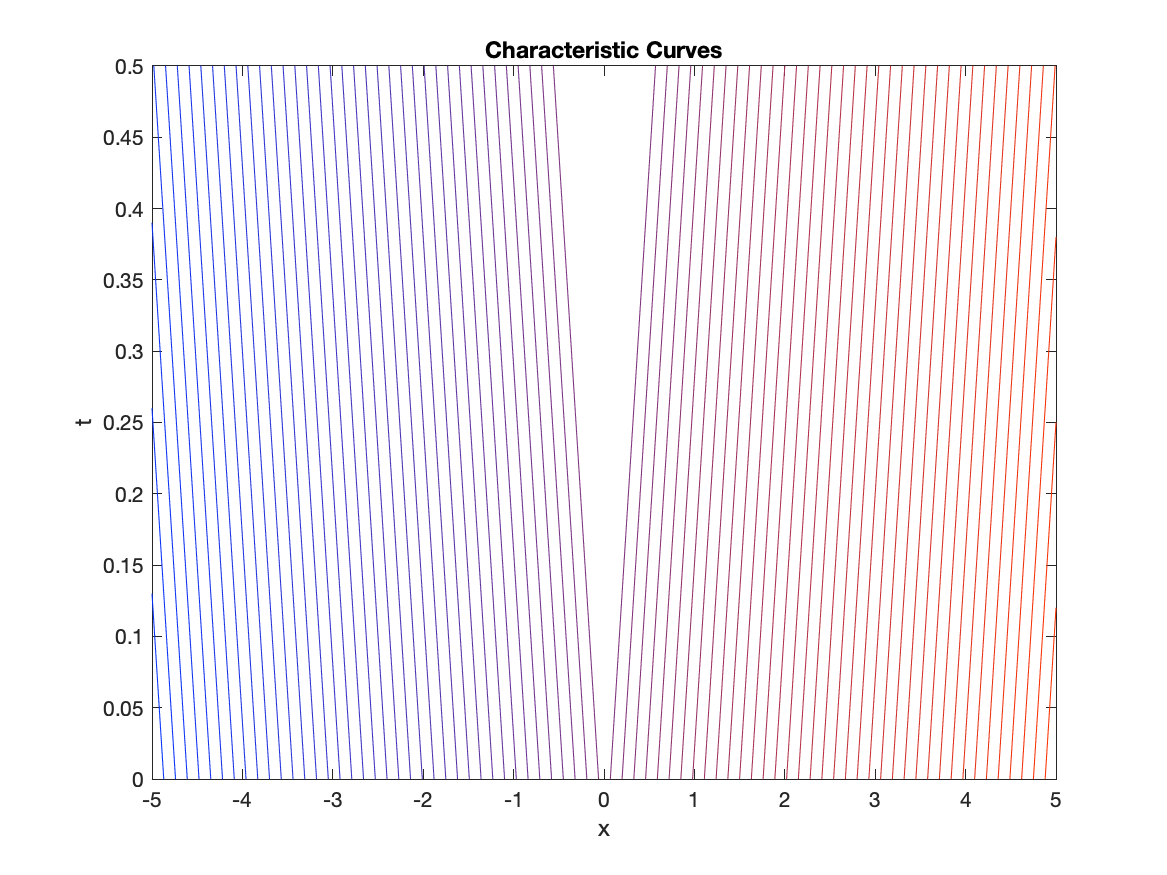
\includegraphics[width=4in]{CharCurves.png}
        \caption{Characteristics of the Burger's Equation}
        \label{fig:CharCurves}
    \end{figure}
    \begin{figure}
        \centering
        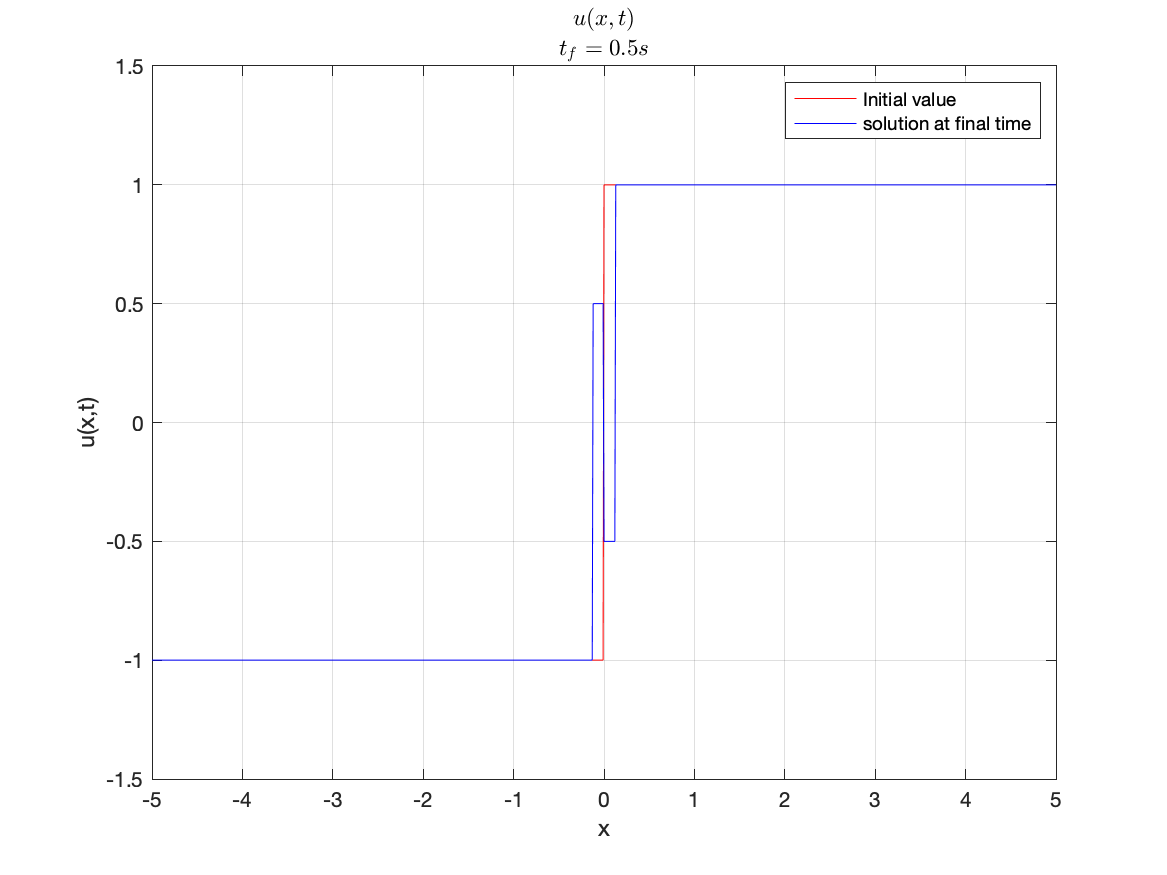
\includegraphics[width=4in]{WeakSol.png}
        \caption{Weak Solution at $t=0\ s$ and at $t=0.5 \ s$ }
        \label{fig:WeakSol}
    \end{figure}
    %%%
    %%%
    %%%
    \item {\color{blue}Construct the entropy satisfying weak solution to this problem.} \\
    I did not know how to construct an entropy stable solution but this is my attempt. From the characteristics we can observe that, there is no shock wave in this problem but more of a refraction fan. So, I did some research and the only physical weak solution to this problem is of the same form as the weak solution presented, except the speeds of propagation used are the respective left velocity and right velocity of the solution itself.
    \begin{align*}
        u(x,t) = 
        \begin{cases}
            u_L,  & x<u_L t, \\
            x/t, & u_Lt\leq x \leq u_R t \\
            u_R,   & x>u_R t
        \end{cases} \\
        u(x,t) = 
        \begin{cases}
            -1,  & x< -t, \\
            x/t, & -t\leq x \leq t \\
            1,   & x> t
        \end{cases}
    \end{align*}
    %%%
    %%%
    %%%
    \item {\color{blue}Create a conservative upwind code to run this case and present computed solution at $t=0.5$. Compare the numerical solution to the exact solution from part (c) above.} \\
    I tried the upwind flux scheme and it was not really converging. Hence, I did some research on my own and the only method I could understand was the Godunov scheme described in the Finite Volume literature. I have tried to attempt the Godunov scheme in my code for multiple initial conditions and it was stable for many initial conditions, even for the one where a shock wave is encountered. The scheme I have written is as follows. \\
    The domain I have considered is $x_1=-5$ to $x_2=5$.
    \begin{align*}
        \dx =& \ (x_2-x_1)/N; \\
        x_j =& \ x_1 + (j+\frac{1}{2})\dx
    \end{align*}
    The solution variables are declared at $x_j$ which is the center of each element. Now, the standard upwind scheme is written as, 
    \begin{align*}
        u^{n+1}_j =& \ u^n_j - \frac{\dt}{\dx}\bra{\Hat{F}^{n}_{j+\frac{1}{2}}\bra{u^n_j,u^n_{j+1}} - \Hat{F}^n_{j-\frac{1}{2}}\bra{u^n_{j+1},u^n_j}} \\
        j =& \ 1,2,3,...,N-1
    \end{align*}
    \begin{align*}
        \Hat{F}^n_{j+\frac{1}{2}}\bra{u_L,u_R} = 
        \begin{cases}
            u_L, & u_L \geq 0\ \text{and}\ u_R \geq 0 \\
            u_R, & u_L \leq 0\ \text{and}\ u_R \leq 0 \\
            u^{*}, & u_L \geq 0\ \text{and}\ u_R \leq 0 \\
            0,   & u_L \leq 0\ \text{and}\ u_R \geq 0
        \end{cases}
    \end{align*}
    Here,
    \begin{align*}
        u^{*} =
        \begin{cases}
            u_L, & \frac{f(u_L)-f(u_R)}{u_L-u_R}\geq 0 \\
            u_R, & \frac{f(u_L)-f(u_R)}{u_L-u_R}\leq 0 
        \end{cases}
    \end{align*}
    Neumann like Boundary conditions are considered at both ends and its given by, 
    \begin{align*}
        u(0) =& u(1) \\
        u(N) =& u(N-1) 
    \end{align*}
    The code is attached in the Listing~\ref{lst:GodunovUpwind}.
    \lstinputlisting[caption={Burger's Equaiton - Upwind Godunov Scheme}, label = {lst:GodunovUpwind}, language=Matlab]{burgersEqn.m}. The comparison of the entropy stable physical solution and the numerical solution is shown in Fig~\ref{fig:GUW}.
    \begin{figure}[htp]
        \centering
        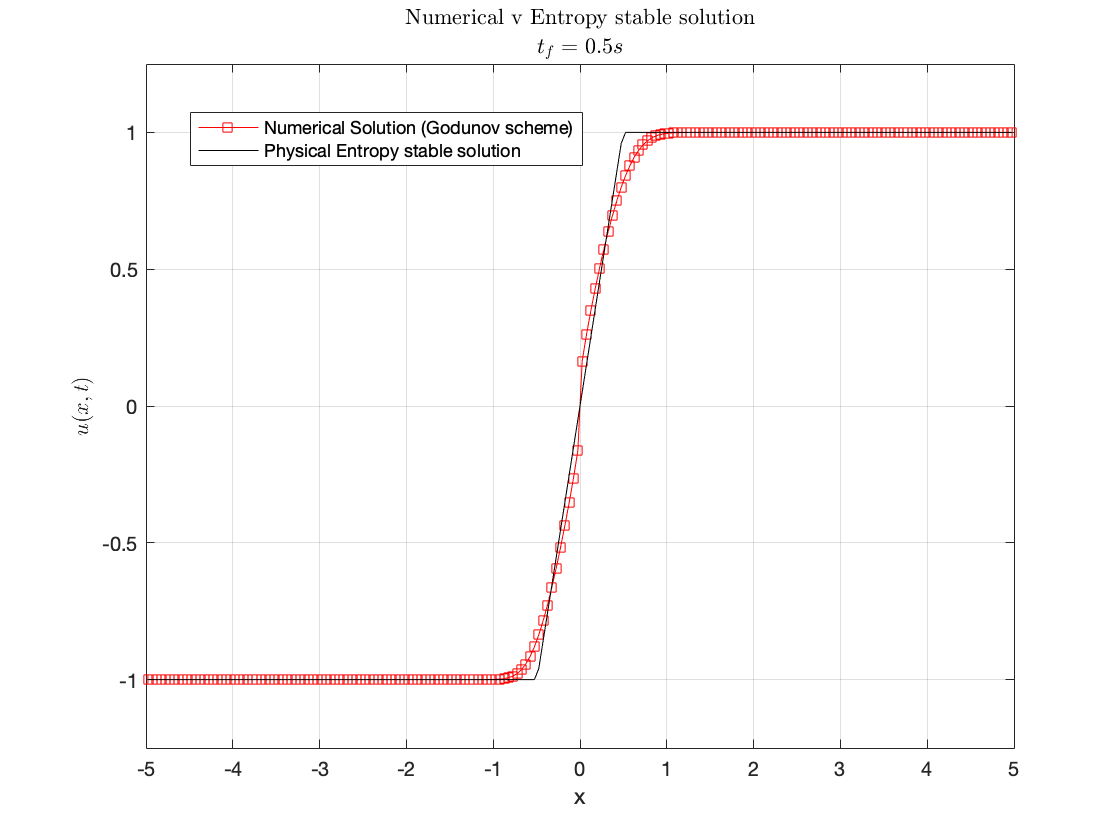
\includegraphics[width=5in]{Godunov_FanSol}
        \caption{Numerical Solution v Entropy Stable weak Solution}
        \label{fig:GUW}
    \end{figure}
  \end{enumerate}
  
  %%%%%
  %%%%%
  %%%%%
  %%%%%
  %%%%%
  \item {\color{red}(20 pts. extra credit) Now let us revisit the annular section problem from PS7, and consider the steady state of a heat conduction problem in an annular section}
  \begin{align*}
    0 = \left[\frac{1}{r}(ru_r)_r+\frac{1}{r^2}u_{\theta\theta}\right], \quad 1<r<2, \quad 0<\theta<\frac{\pi}{2},
  \end{align*}
  {\color{red}with boundary conditions}
  \begin{align*}
    u_r(1,\theta) = 0, \qquad & u_r(2,\theta) = 0 \\
    u(r,0) = 0 \qquad & u(r,\frac{\pi}{2}) = (r-1)^2(r-2)^2.
  \end{align*}
  
  \begin{enumerate}
    %%%
    %%%
    %%%
    \item {\color{blue}Starting from your code from PS7 (or the one from SS7), write a second-order accurate code to solve this problem using centered differencing. Hint, as before you may find it useful to use manufactured solutions to verify the accuracy of your code.}
    \begin{align*}
        r_j =& \ r_1 + j\Delta r & j=& -1,0,1,\ldots \ldots N_r+1\\
        \theta_k =& \ \theta_1 + k\Delta \theta & k=& -1,0,1,\ldots \ldots N_\theta +1
    \end{align*}
    \begin{align*}
        \frac{1}{r_{j,k}}\frac{r_{j+\frac{1}{2},k}v_{j+1,k}-\bra{r_{j+\frac{1}{2},k}+r_{j-\frac{1}{2},k}}v_{j,k}+r_{j-\frac{1}{2},k}v_{j-1,k} }{\Delta r^2}+& \\
        \frac{1}{r_{j,k}^2}\frac{v_{j,k+1}-2v_{j,k}+v_{j,k-1}}{\Delta \theta^2} =& \ 0
    \end{align*}
    The Boundary conditions are writen as,
    \begin{align*}
        \frac{v_{2,k}-v_{-1,k}}{2\Delta r} =& \ 0, & \frac{v_{N_r+1,k}-v_{N_r-1,k}}{2\Delta r} =& \ 0 \\
        \frac{v_{j,-1}+v_{j,2}}{2} =& 0, & \frac{v_{j,N_\theta-1}+v_{j,N_\theta+1}}{2} =& \ (r_{j,\theta_2}-1)^2(r_{j,\theta_2}-2)^2
    \end{align*}
    This is written in a matrix form as follows,
    \begin{align*}
        {\bf \underline{\underline{A}}} \ \underline{v} = \underline{0}
    \end{align*}
    This discretization is tested against the manufactured solution, 
    \begin{align*}
        u(r,\theta) =& \ (r-1)^2(r-2)^2 \sin(\theta)
    \end{align*}
    where, the PDE becomes,
    \begin{align*}
        \bra{\frac{1}{r}\bra{ru_r}_r+\frac{1}{r^2}u_{\theta \theta}} =& \ f(r,\theta) 
    \end{align*}
    The error convergence can be seen in Fig~\ref{fig:ErrPlotQ2}. The code is attached in Listing~\ref{lst:HE2DSS}.
    \lstinputlisting[caption={Heat Equation 2D - Steady State, Mapping}, label={lst:HE2DSS},language=Matlab]{HeatEqn2DSteady.m}.
    \begin{figure}[htp]
        \centering
        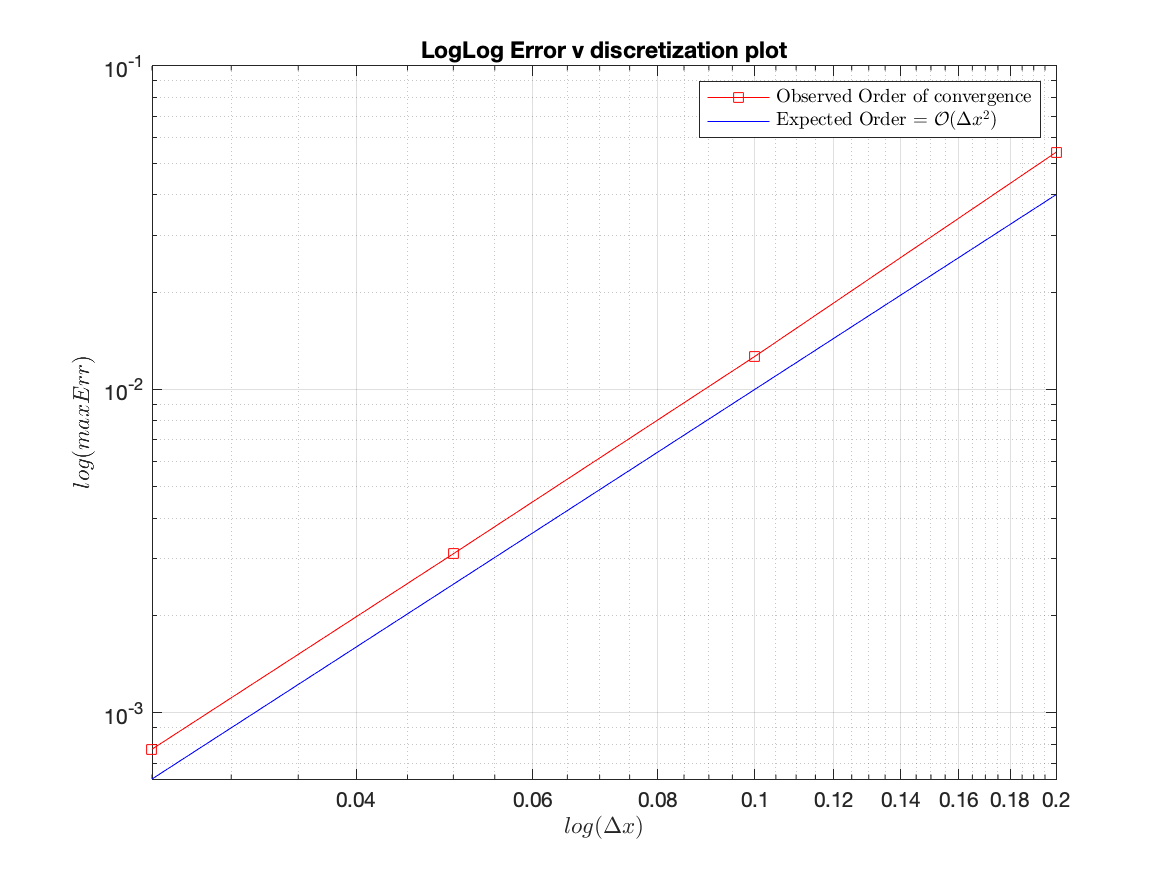
\includegraphics[width=5in]{ErrPlotQ2}
        \caption{Error Convergence plot}
        \label{fig:ErrPlotQ2}
    \end{figure}
    %%%
    %%%
    %%%
    \item {\color{blue}Using 40 grid lines in both the radial and angular coordinate directions, compute a numerical solutions to this problem, and create a surface plots of the solution. In addition, create a single line plot with two curves showing the solution along the inner radius ($r=1$), and the outer radius ($r=2$), as a function of $\theta$.} \\
    I have written down two iterative solvers. Three cases are shown in the following figures Fig~\ref{fig:P_Jacobi}, Fig~\ref{fig:P_GS} and Fig~\ref{fig:P_Inv}. The Iterative solver code is attached in Listing~\ref{lst:IS}. The matrix $\matA{A}$ is first separated into the Lower diagonal ($\matA{L}$), Diagonal ($\matA{D}$) and upper diagonal ($\matA{U}$) matrices.
    \lstinputlisting[caption={Iterative Solver Function Handle},label={lst:IS},language=Matlab]{IterativeSolver.m}.
    \begin{itemize}
        \item {\bf Jacobi}: Tolerance $\varepsilon = 1e-3 $ and Max Iterations = 3000 
        \begin{align*}
            \underline{u}^{n+1} =& \ \matA{D}^{-1} \ \underline{b} - \matA{D}^{-1}\bra{\matA{L}+\matA{U}} \\
            \matA{R} =& \ \matA{A}\ \underline{u}^{n+1}- \underline{b}
        \end{align*}
        This is done until the norm of the Residual $\matA{R}$ gets below $\varepsilon$ or until max iterations are reached.
        \item {\bf Gauss-Siedel}: Tolerance $\varepsilon = 1e-3 $ and Max Iterations = 3000 
        \begin{align*}
            \matA{L^{*}} =& \ \matA{L} + \matA{D}\\
            \underline{u}^{n+1} =& \ \matA{L^{*}}^{-1} \ \underline{b} - \matA{L^{*}}^{-1}\matA{U} \\
            \matA{R} =& \ \matA{A}\ \underline{u}^{n+1}- \underline{b}
        \end{align*}
        This is done until the norm of the Residual $\matA{R}$ gets below $\varepsilon$ or until max iterations are reached.
        \item {\bf Direct}: A direct solver is used and its computed as $\underline{u} = \matA{A}^{-1}\ \underline{b}$.
    \end{itemize}
    \begin{figure}[htp]
        \centering
        \begin{tabular}{cc}
            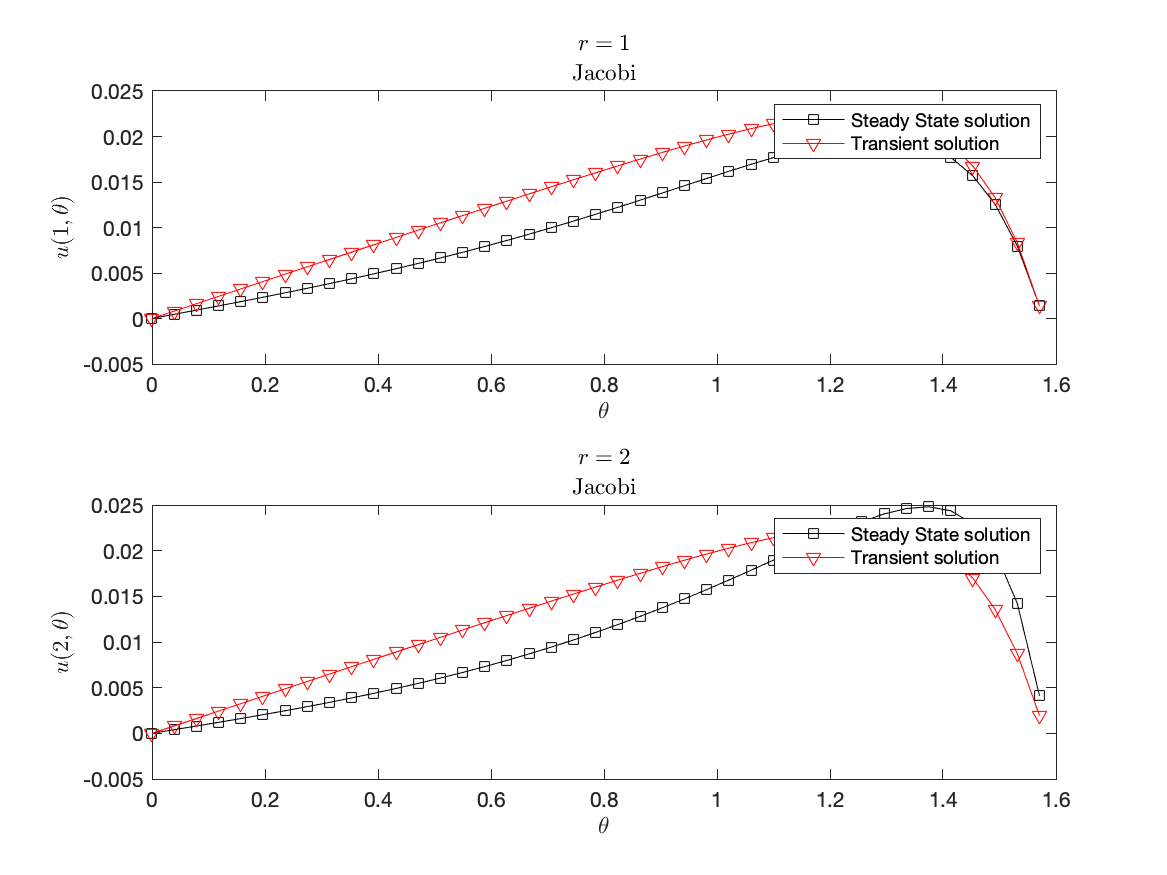
\includegraphics[width=3.5in]{p11} & 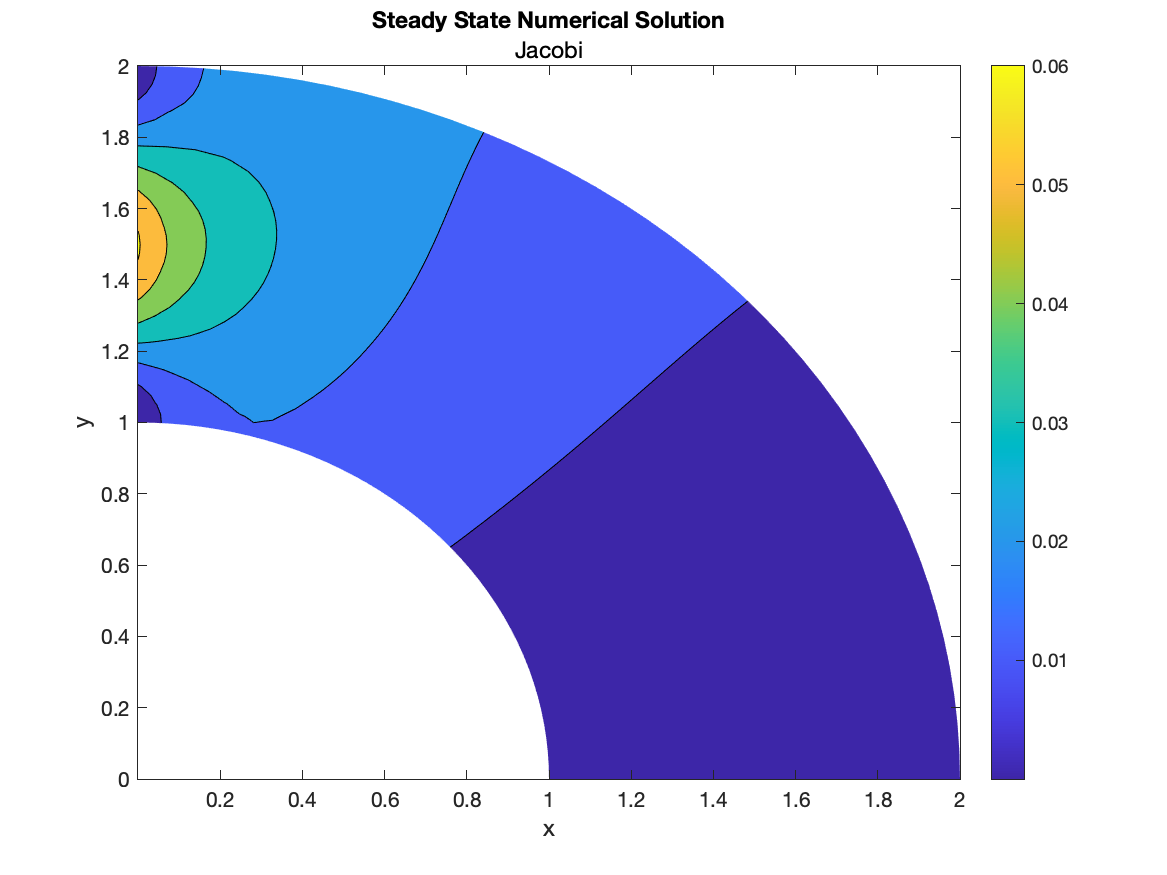
\includegraphics[width=3.5in]{p21} \\ 
            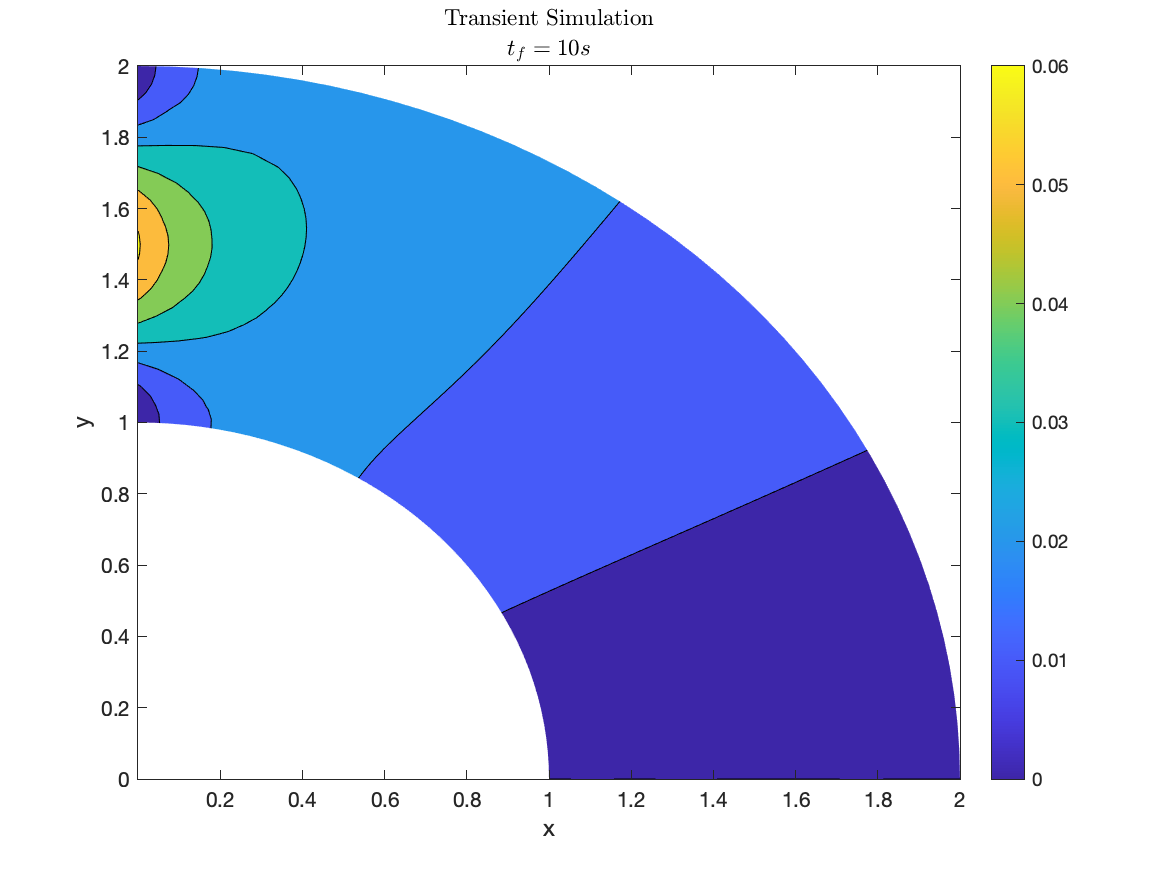
\includegraphics[width=3.5in]{p31} & 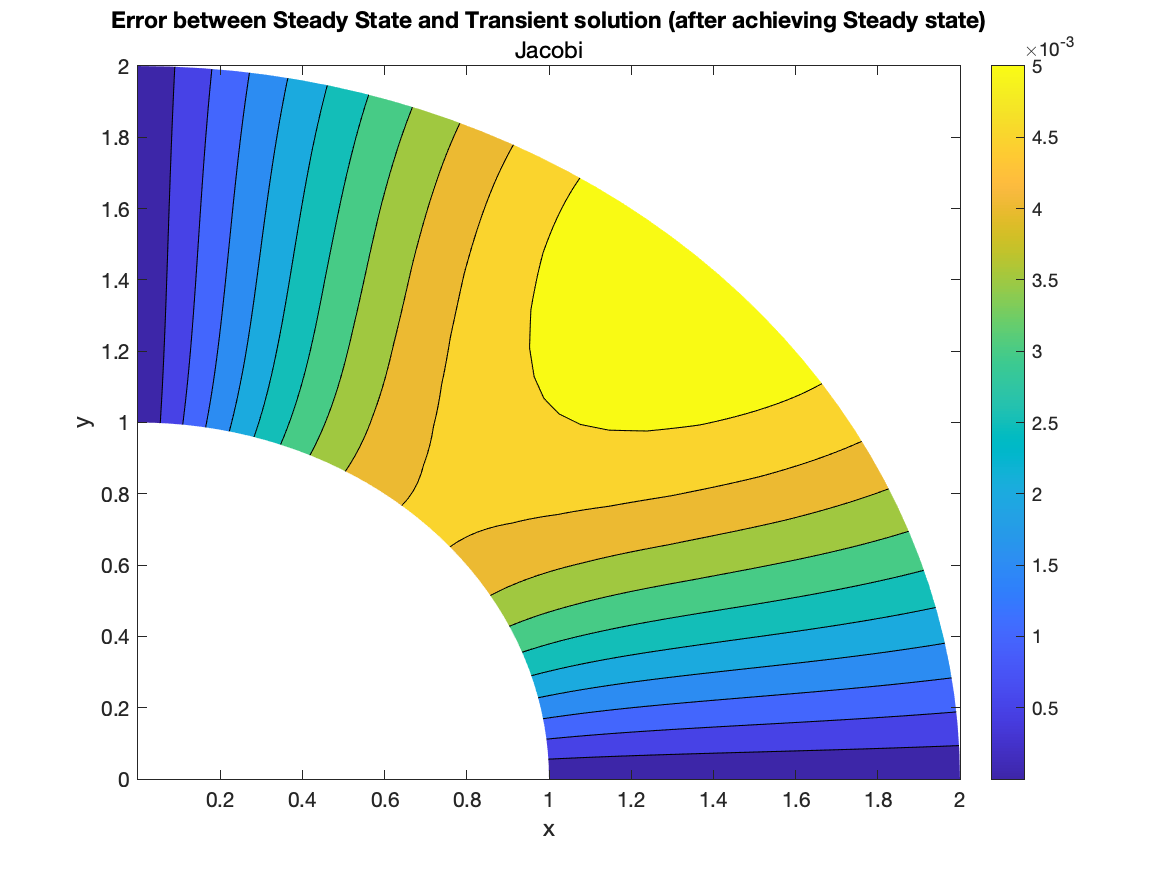
\includegraphics[width=3.5in]{p41}
        \end{tabular}
        \caption{Jacobi Iterative solver results}
        \label{fig:P_Jacobi}
    \end{figure}
    \begin{figure}[htp]
        \centering
        \begin{tabular}{cc}
            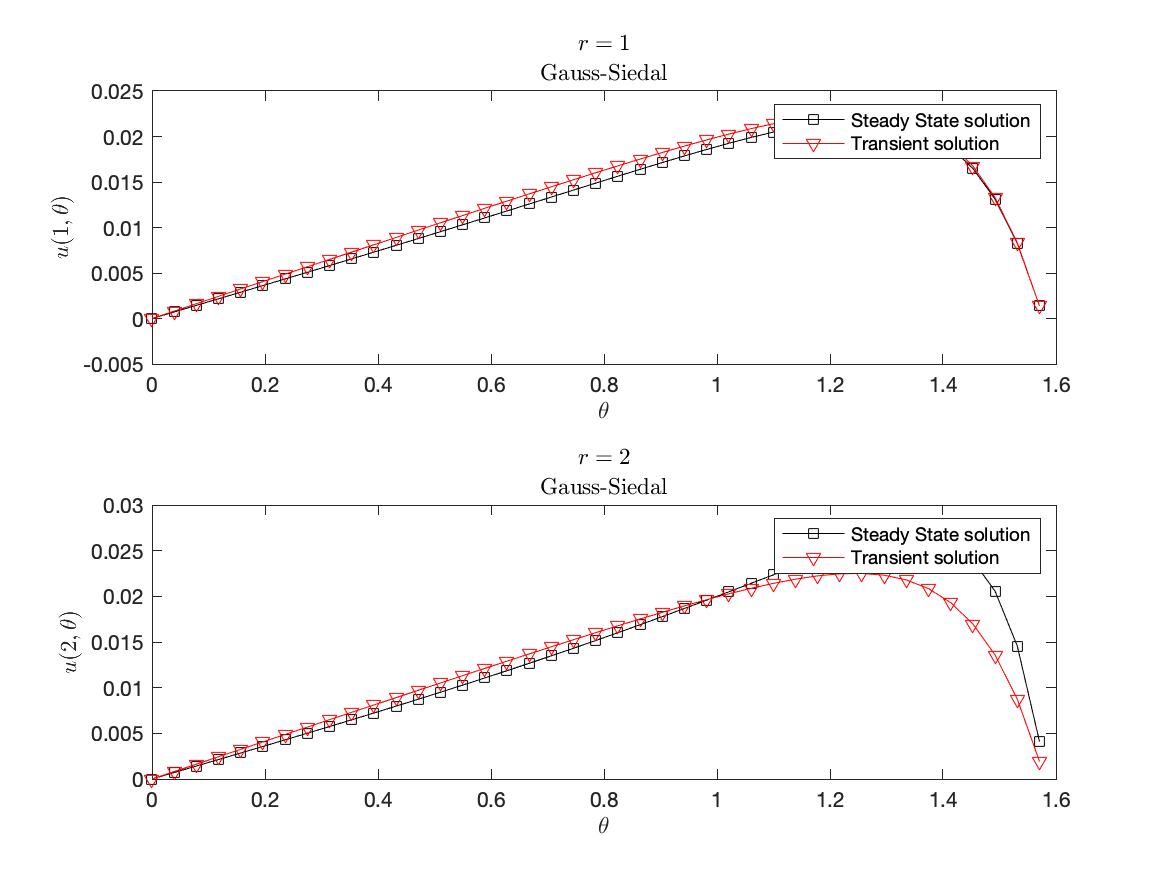
\includegraphics[width=3.5in]{p12} & 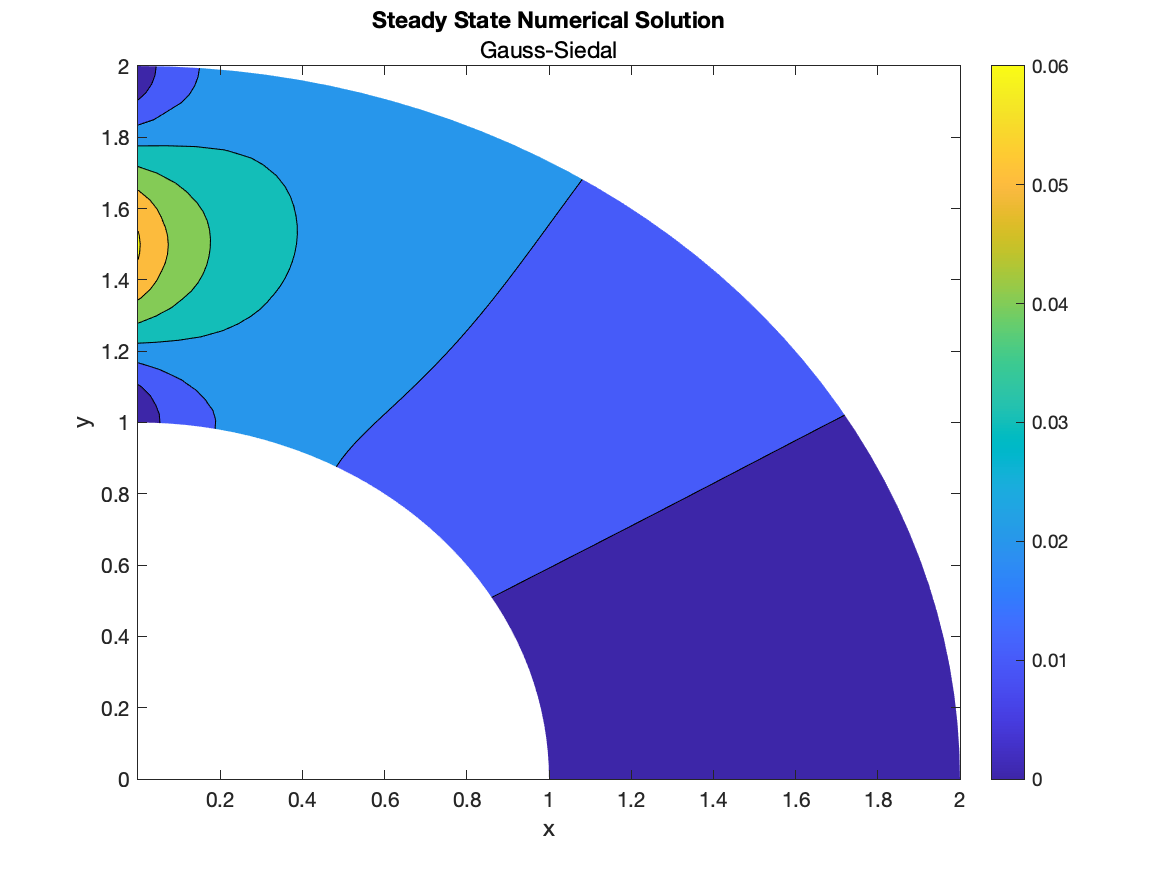
\includegraphics[width=3.5in]{p22} \\ 
            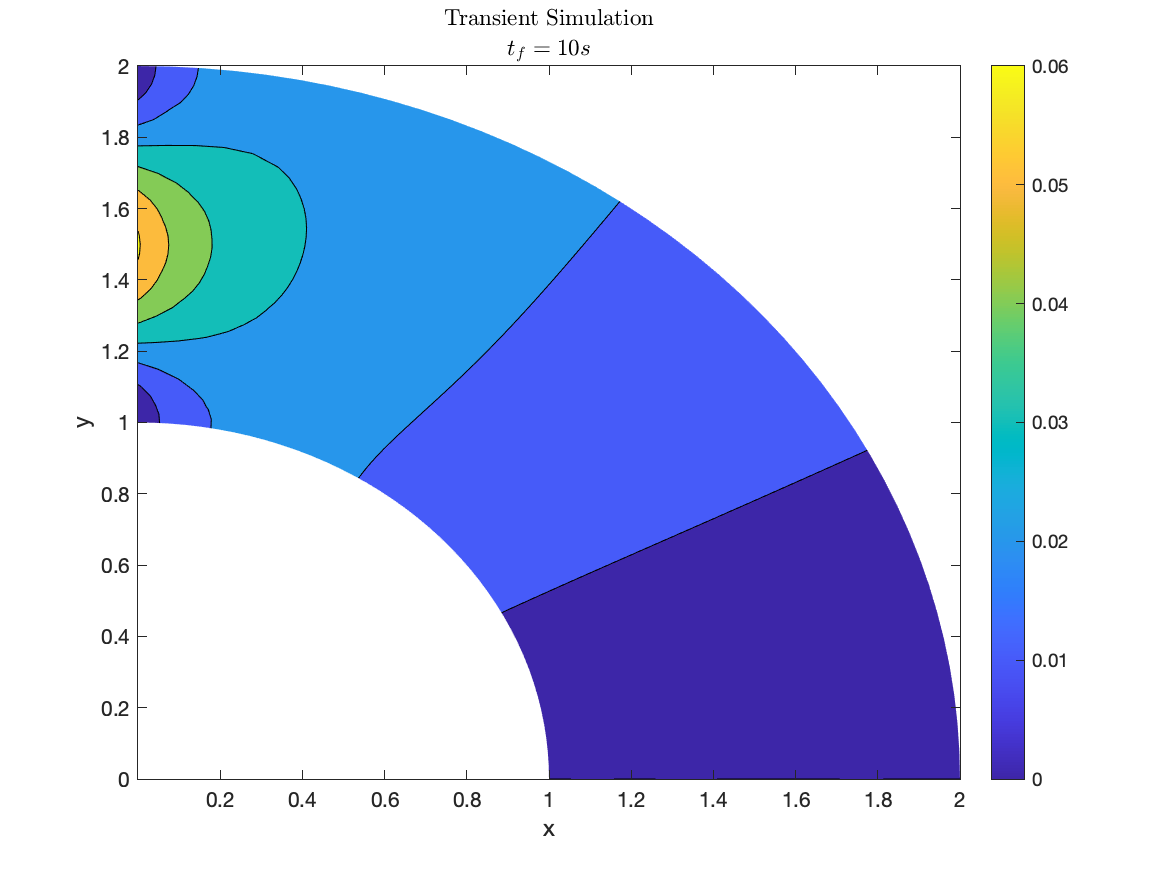
\includegraphics[width=3.5in]{p32} & 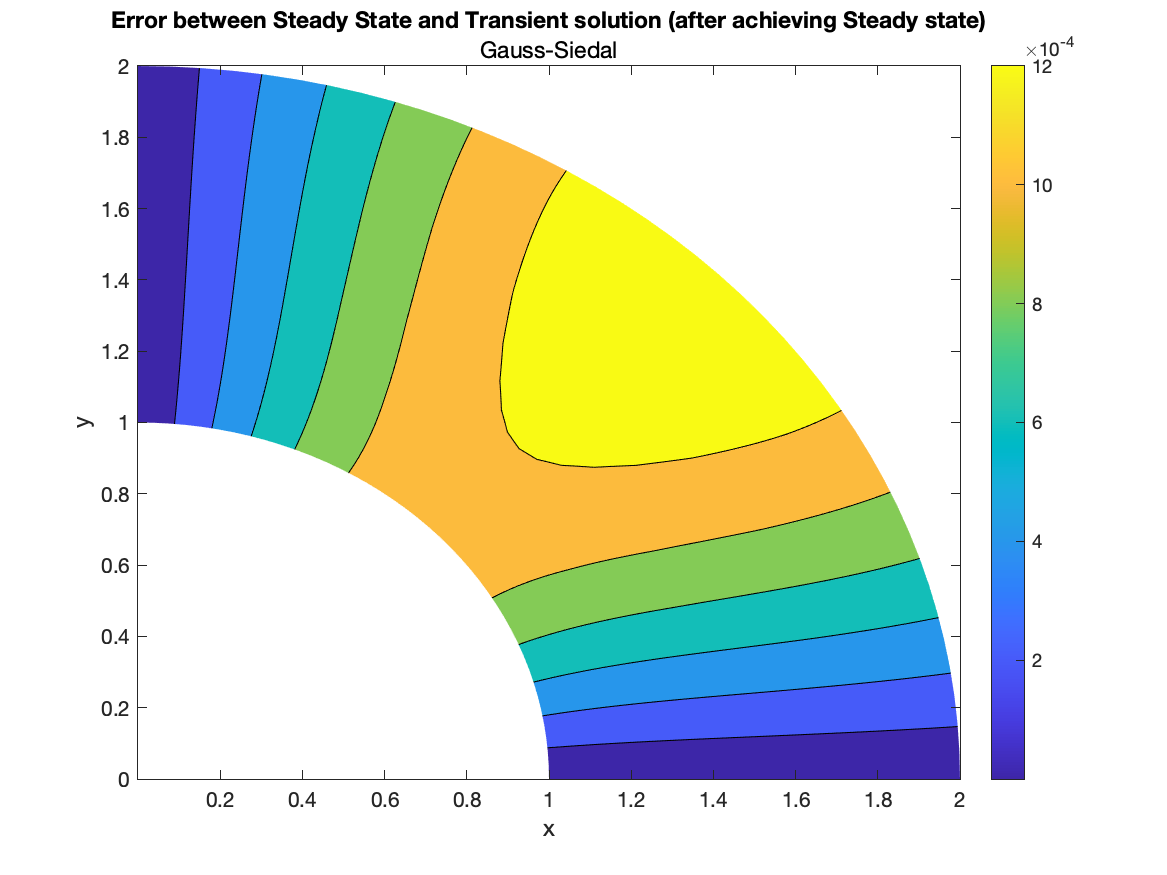
\includegraphics[width=3.5in]{p42}
        \end{tabular}
        \caption{Gauss Siedal Iterative solver results}
        \label{fig:P_GS}
    \end{figure}
    \begin{figure}[htp]
        \centering
        \begin{tabular}{cc}
            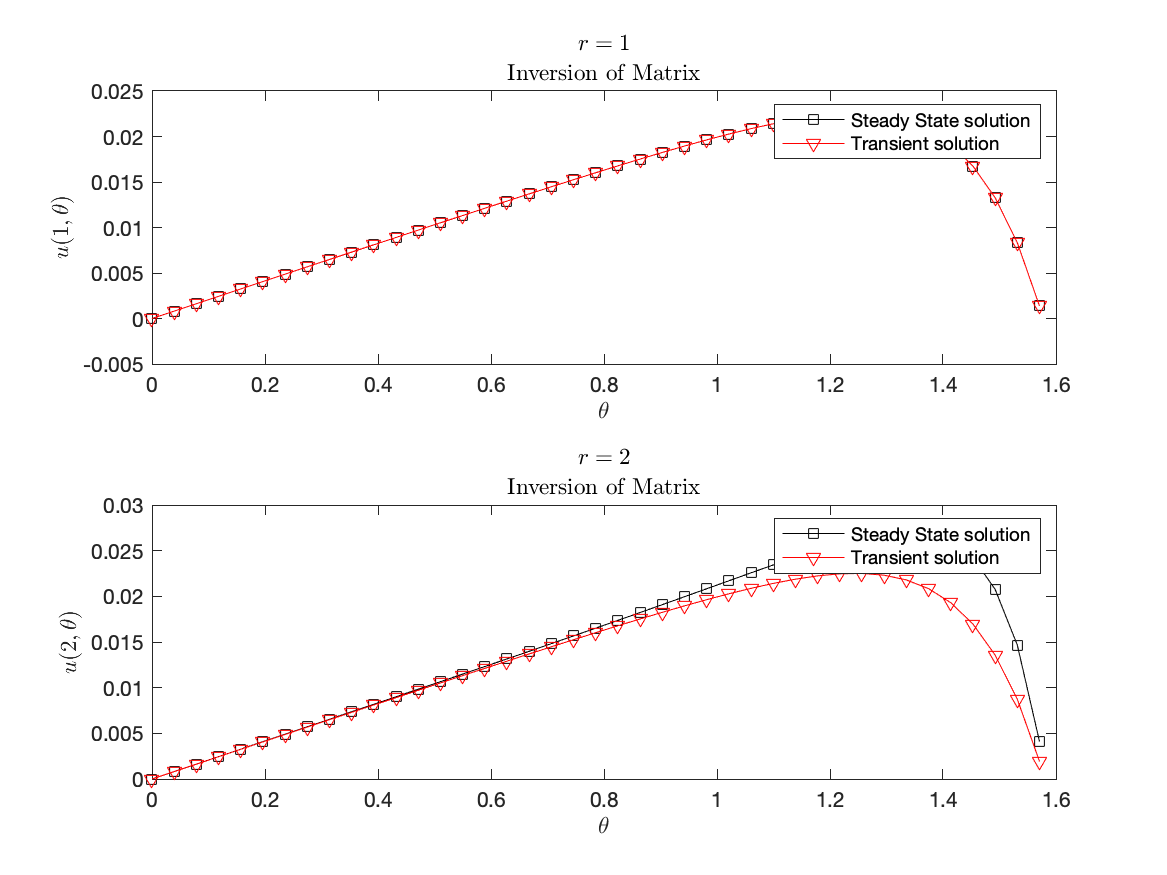
\includegraphics[width=3.5in]{p13} & 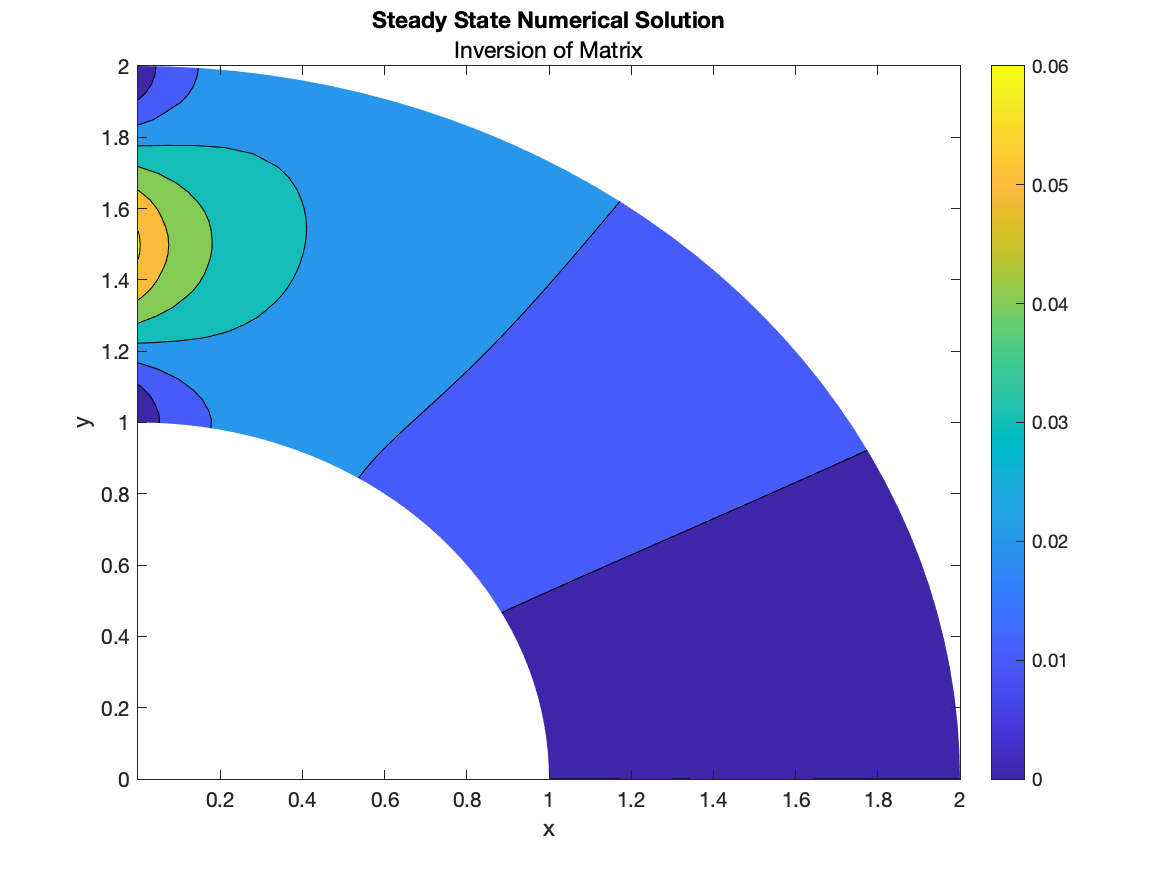
\includegraphics[width=3.5in]{p23} \\ 
            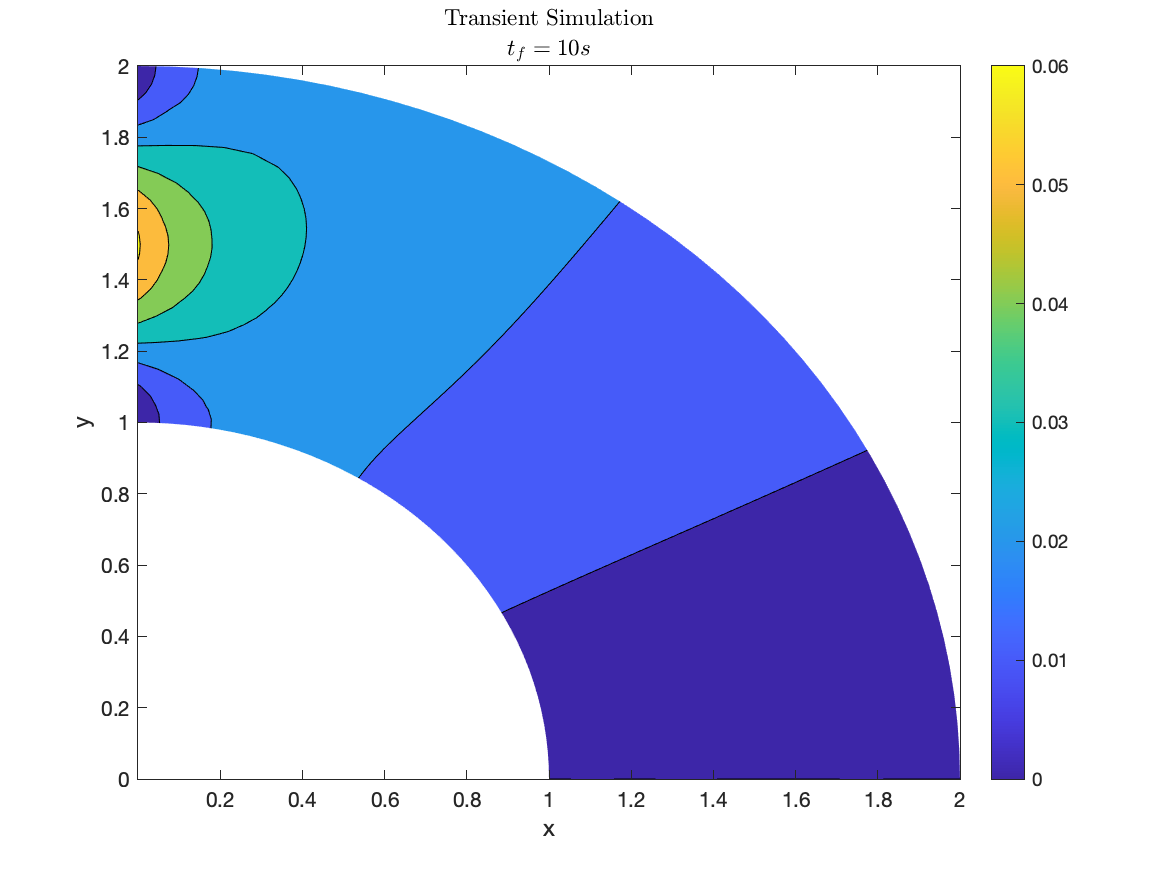
\includegraphics[width=3.5in]{p33} & 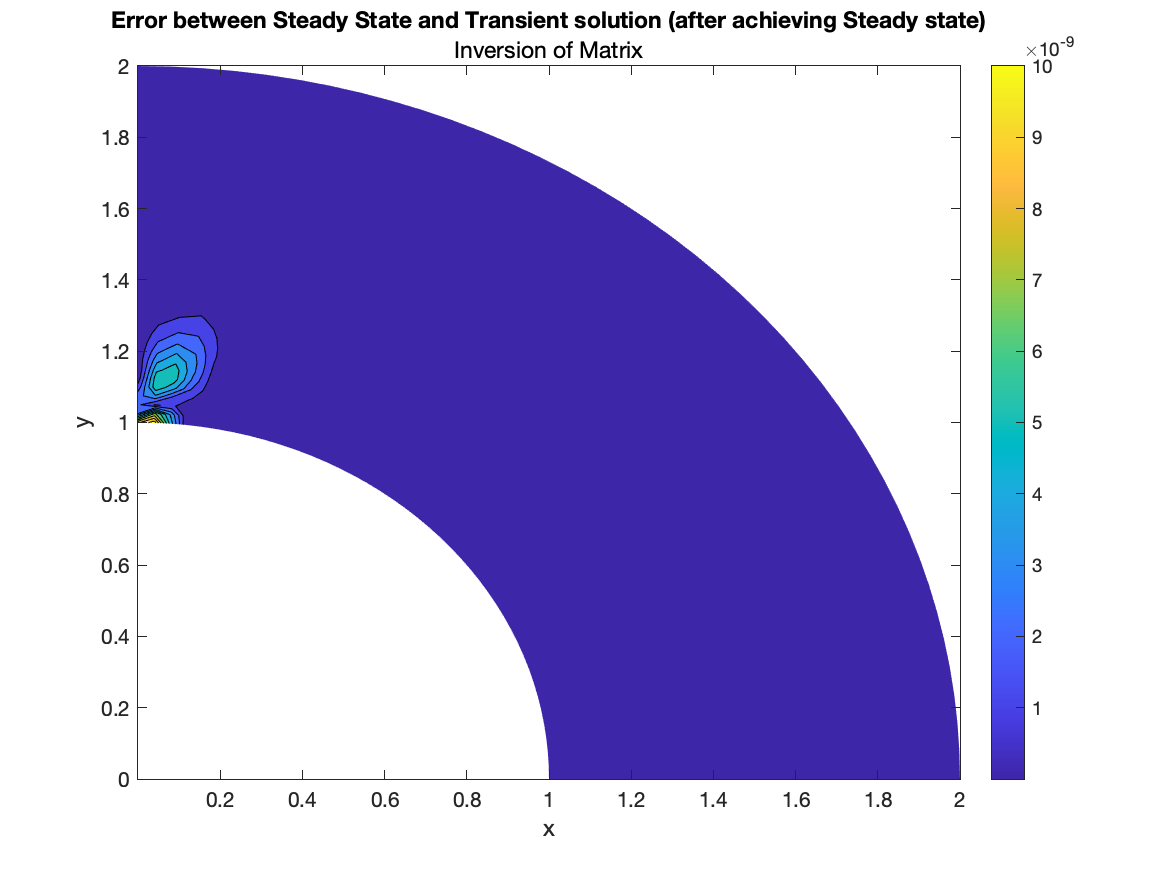
\includegraphics[width=3.5in]{p43}
        \end{tabular}
        \caption{Inversion results}
        \label{fig:P_Inv}
    \end{figure}
    %%%
    %%%
    %%%
    \item {\color{blue}Finally, compare the steady state solution you compute here to the solutions of the time-dependent problem from PS7. In particular show the approach of the time-dependent solutions to the steady solution along the inner radius $r=1$.} \\
    The comparison at $r=1$ are also plotted in Fig~\ref{fig:P_Jacobi}, Fig~\ref{fig:P_GS} and Fig~\ref{fig:P_Inv}. The results of the transient simulation at $r=1$ seems to agree better with the steady state results as opposed to the solutions at the inner radius $r=2$.
  \end{enumerate}
\end{enumerate}
\end{document}